\RequirePackage[l2tabu, orthodox]{nag}

%\documentclass[]{article}
\documentclass[11pt]{scrartcl}
\usepackage[usename, dvipsnames]{xcolor}
\usepackage[pdfencoding=auto]{hyperref}
\usepackage[msc-links]{amsrefs}
\usepackage{cleveref} % use \cref{}, automatically deduces theorem, proposition, etc
\usepackage[mathletters]{ucs}
\usepackage[utf8]{inputenc}
\usepackage[T1]{fontenc}
\usepackage{datetime}

\usepackage{array}
\usepackage{mathtools}
\usepackage{amsmath, amsthm, amssymb, amsfonts, amsxtra, amscd, thmtools}
\let\proof\relax
\let\endproof\relax

% Boxes around theorem environments.
\usepackage[many]{tcolorbox}

\usepackage{color}
%\usepackage{unicode-math}
\usepackage{newunicodechar}
\newunicodechar{ε}{\varepsilon}
\newunicodechar{δ}{\delta}
\newunicodechar{µ}{\mu}
\newunicodechar{→}{\to}
\newunicodechar{≤}{\leq}
\newunicodechar{∈}{\in}
\newunicodechar{⊆}{\subseteq}
\newunicodechar{Λ}{\Lambda}
\newunicodechar{∞}{\infty}
\newunicodechar{×}{\times}
\everymath{\displaystyle}



\usepackage{microtype}
\usepackage[pdfencoding=auto]{hyperref}
\usepackage{bookmark}
\usepackage{booktabs}
\usepackage{todonotes}
\usepackage[msc-links]{amsrefs}
\usepackage{cleveref} % use \cref{}, automatically deduces theorem, proposition, etc
\usepackage{csquotes}
\usepackage{longtable}
\usepackage{tabularx}
\usepackage{bbm}
% Creating multiple types of index
\usepackage{imakeidx}

% Remove indentation for new paragraphs
\usepackage{parskip}
% But leave space before amsthm environments
\makeatletter
\def\thm@space@setup{%
  \thm@preskip=2em
  \thm@postskip=2em
}
\makeatother


\usepackage{stmaryrd}
\usepackage{adjustbox}
\usepackage{centernot}
% \centernot\whatever


% Better indicator function
\usepackage{bbm}
\newcommand{\indic}[1]{\mathbbm{1} \left[ {#1} \right] }

% Highlight quote
\usepackage{environ}
\definecolor{camel}{rgb}{0.76, 0.6, 0.42}
\definecolor{babyblue}{rgb}{0.54, 0.81, 0.94}
\definecolor{block-gray}{gray}{0.85}
\NewEnviron{myblock}
{\colorbox{block-gray}{%
\parbox{\dimexpr\linewidth-2\fboxsep\relax}{%
\small\addtolength{\leftskip}{10mm}
\addtolength{\rightskip}{10mm}
\BODY}}
}
\renewcommand{\quote}{\myblock}
\renewcommand{\endquote}{\endmyblock}

% Nice math font that journals use
%\usepackage[lite]{mtpro2}
%\usepackage{mathrsfs}
%\usepackage{mathptmx}
\usepackage{lmodern}
%\usepackage[sc]{mathpazo}

% Theorem Styles
\usepackage[framemethod=tikz]{mdframed}

\theoremstyle{definition}
\newtheorem{exercise}{Exercise}[section]
\newtheorem{solution}{Solution}

% Theorem Style
\newtheoremstyle{theorem}% name
  {0em}%         Space above, empty = `usual value'
  {1em}%         Space below
  {\normalfont}% Body font
  {\parindent}%         Indent amount (empty = no indent, \parindent = para indent)
  {\bfseries}% Thm head font
  {.}%        Punctuation after thm head
  {\newline}% Space after thm head: \newline = linebreak
  {\thmname{#1}\thmnumber{ #2}\thmnote{\itshape{(#3)}}}%
\theoremstyle{theorem}
\tcolorboxenvironment{theorem}{
  boxrule=0pt,
  boxsep=0pt,
  breakable,
  enhanced jigsaw,
  fonttitle={\large\bfseries},
  opacityback=0.8,
  colframe=cyan,
  borderline west={4pt}{0pt}{orange},
  attach title to upper={}
}
\newtheorem{theorem}{Theorem}[section]

% Proposition Style
\tcolorboxenvironment{proposition}{
  boxrule=1pt,
  boxsep=0pt,
  breakable,
  enhanced jigsaw,
  opacityback=0.0,
  colframe=cyan
}
\newtheorem{proposition}[theorem]{Proposition}
\tcolorboxenvironment{lemma}{
  boxrule=1pt,
  boxsep=0pt,
  breakable,
  enhanced jigsaw,
  opacityback=0.2,
  colframe=cyan
}
\newtheorem{lemma}[theorem]{Lemma}
% Claim
\tcolorboxenvironment{claim}{
  boxrule=1pt,
  boxsep=0pt,
  breakable,
  enhanced jigsaw,
  opacityback=0.2,
  colframe=cyan
}
\newtheorem{claim}[theorem]{Claim}


% Corollary
\tcolorboxenvironment{corollary}{
  colback=cyan,
  boxrule=1pt,
  boxsep=0pt,
  breakable,
  enhanced jigsaw,
  opacityback=0.1,
  colframe=cyan
}
\newtheorem{corollary}[theorem]{Corollary}

% Proof Style
\newtheoremstyle{proof}% name
  {0em}%         Space above, empty = `usual value'
  {2em}%         Space below
  {\normalfont}% Body font
  {\parindent}%         Indent amount (empty = no indent, \parindent = para indent)
  {\itshape}% Thm head font
  {.}%        Punctuation after thm head
  {\newline}% Space after thm head: \newline = linebreak
  {\thmname{#1} \thmnote{\itshape{(#3)}}}%         Thm head spec
\theoremstyle{proof}
\tcolorboxenvironment{proof}{
  colback=camel,
  opacityfill=0.25,
  boxrule=1pt,
  boxsep=0pt,
  breakable,
  enhanced jigsaw
}
\newtheorem*{pf}{Proof}
\newenvironment{proof}
{\pushQED{$\qed$}\pf}
{\par\popQED\endpf}

% Definition Style
\newtheoremstyle{definition}% name
  {0em}%         Space above, empty = `usual value'
  {2em}%         Space below
  {\normalfont}% Body font
  {\parindent}%         Indent amount (empty = no indent, \parindent = para indent)
  {\bfseries}% Thm head font
  {.}%        Punctuation after thm head
  {\newline}% Space after thm head: \newline = linebreak
  {}%         Thm head spec
\theoremstyle{definition}
\tcolorboxenvironment{definition}{
  colback=babyblue,
  boxrule=0pt,
  boxsep=0pt,
  opacityfill=0.45,
  breakable,
  enhanced jigsaw,
  borderline west={4pt}{0pt}{blue},
  colbacktitle={babyblue},
  coltitle={black},
  fonttitle={\large\bfseries},
  attach title to upper={},
}
\newtheorem{definition}{Definition}[theorem]

% Break Environment
\makeatletter
\newtheoremstyle{break}% name
  {}%         Space above, empty = `usual value'
  {2em}%         Space below
  {
    \addtolength{\@totalleftmargin}{2.5em}
    \addtolength{\linewidth}{-2.5em}
    \parshape 1 2.5em \linewidth
  }% Body font
  {}%         Indent amount (empty = no indent, \parindent = para indent)
  {\bfseries}% Thm head font
  {.}%        Punctuation after thm head
  {\newline}% Space after thm head: \newline = linebreak
  {}%         Thm head spec
\makeatother

\theoremstyle{break}
\newtheorem{example}{Example}[section]

% Problem Style
\newtheoremstyle{problem} % name
  {0em}                   % Space above, empty = `usual value'
  {2em}                   % Space below
  {\normalfont}           % Body font
  {\parindent}            % Indent amount (empty = no indent, \parindent = para indent)
  {\itshape}              % Thm head font
  {}                      % Punctuation after thm head
  {\newline}              % Space after thm head: \newline = linebreak
  {\thmnote{\itshape{(#3)}}}     % Thm head spec
\theoremstyle{problem}
\tcolorboxenvironment{problem}{
  boxrule=1pt,
  boxsep=0pt,
  breakable,
  enhanced jigsaw,
  opacityback=0.0,
  colframe=cyan
}
\newtheorem{problem}{Problem}


%Pagination stuff.
\setlength{\topmargin}{-.3 in}
\setlength{\oddsidemargin}{0in}
\setlength{\evensidemargin}{0in}
\setlength{\textheight}{9.in}
\setlength{\textwidth}{6.5in}
% \pagestyle{empty} %removes page numbers.

% Inkscape figures from Vim
\usepackage{import}
\usepackage{pdfpages}
\usepackage{transparent}

\newcommand{\incfig}[1]{%
    \def\svgwidth{\columnwidth}
    \import{./figures/}{#1.pdf_tex}
}
%\pdfsuppresswarningpagegroup=1

% Pandoc-specific fixes
\providecommand{\tightlist}{%
  \setlength{\itemsep}{0pt}\setlength{\parskip}{0pt}}

% Tikz and Graphics
\usepackage{amscd}
\usepackage{tikz}
\usetikzlibrary{arrows, arrows.meta, cd, fadings, patterns, calc, decorations.markings, matrix, positioning}
\tikzfading[name=fade out, inner color=transparent!0, outer color=transparent!100]
\usepackage{pgfplots}
\pgfplotsset{compat=1.16}
\usepackage[inline]{asymptote}
\usepackage{tikz-layers}

%\usepackage{nath}
%\delimgrowth=1
\DeclarePairedDelimiter\qty{(}{)}

% Major Macros
\usepackage{graphicx}
\usepackage{float}
\DeclareFontFamily{U}{mathx}{\hyphenchar\font45}
\DeclareFontShape{U}{mathx}{m}{n}{
      <5> <6> <7> <8> <9> <10>
      <10.95> <12> <14.4> <17.28> <20.74> <24.88>
      mathx10
      }{}
\DeclareSymbolFont{mathx}{U}{mathx}{m}{n}
\DeclareMathSymbol{\bigtimes}{1}{mathx}{"91}

% Wide tikz equations
\newsavebox{\wideeqbox}
\newenvironment{wideeq}
  {\begin{displaymath}\begin{lrbox}{\wideeqbox}$\displaystyle}
  {$\end{lrbox}\makebox[0pt]{\usebox{\wideeqbox}}\end{displaymath}}



% Fancy chapter headers and footers
\usepackage{fancyhdr}

\pagestyle{fancy}
\fancyhf{}
\fancyhead[LE,RO]{\title}
\fancyhead[RE,LO]{\rightmark}
\fancyfoot[CE,CO]{\leftmark}
\fancyfoot[LE,RO]{\thepage}

\renewcommand{\headrulewidth}{2pt}
\renewcommand{\footrulewidth}{1pt}

% List of Theorems Attempt
\usepackage{etoolbox}
\makeatletter
\patchcmd\thmtlo@chaptervspacehack
  {\addtocontents{loe}{\protect\addvspace{10\p@}}}
  {\addtocontents{loe}{\protect\thmlopatch@endchapter\protect\thmlopatch@chapter{\thechapter}}}
  {}{}
\AtEndDocument{\addtocontents{loe}{\protect\thmlopatch@endchapter}}
\long\def\thmlopatch@chapter#1#2\thmlopatch@endchapter{%
  \setbox\z@=\vbox{#2}%
  \ifdim\ht\z@>\z@
    \hbox{\bfseries\chaptername\ #1}\nobreak
    #2
    \addvspace{10\p@}
  \fi
}
\def\thmlopatch@endchapter{}

\makeatother
\renewcommand{\thmtformatoptarg}[1]{ -- #1}
%\renewcommand{\listtheoremname}{List of definitions}

\newcommand{\ext}{\operatorname{Ext}}
\newcommand{\Ext}{\operatorname{Ext}}
\def\Endo{\operatorname{End}}
\def\Ind{\operatorname{Ind}}
\def\ind{\operatorname{Ind}}
\def\coind{\operatorname{Coind}}
\def\Res{\operatorname{Res}}
\def\Hol{\operatorname{Hol}}
\def\res{\operatorname{Res}}
\def\endo{\operatorname{End}}
\def\ind{\operatorname{Ind}}
\renewcommand{\AA}[0]{{\mathbb{A}}}
\DeclareMathOperator{\Exists}{\exists}
\DeclareMathOperator{\Forall}{\forall}
\newcommand{\Af}[0]{{\mathbb{A}}}
\newcommand{\CC}[0]{{\mathbb{C}}}
\newcommand{\CP}[0]{{\mathbb{CP}}}
\newcommand{\DD}[0]{{\mathbb{D}}}
\newcommand{\FF}[0]{{\mathbb{F}}}
\newcommand{\GF}[0]{{\mathbb{GF}}}
\newcommand{\GG}[0]{{\mathbb{G}}}
\newcommand{\HH}[0]{{\mathbb{H}}}
\newcommand{\HP}[0]{{\mathbb{HP}}}
\newcommand{\KK}[0]{{\mathbb{K}}}
\newcommand{\kk}[0]{{\Bbbk}}
\newcommand{\bbm}[0]{{\mathbb{M}}}
\newcommand{\NN}[0]{{\mathbb{N}}}
\newcommand{\OP}[0]{{\mathbb{OP}}}
\newcommand{\PP}[0]{{\mathbb{P}}}
\newcommand{\QQ}[0]{{\mathbb{Q}}}
\newcommand{\RP}[0]{{\mathbb{RP}}}
\newcommand{\RR}[0]{{\mathbb{R}}}
\newcommand{\SpSp}[0]{{\mathbb{S}}}
\renewcommand{\SS}[0]{{\mathbb{S}}}
\newcommand{\TT}[0]{{\mathbb{T}}}
\newcommand{\ZZ}[0]{{\mathbb{Z}}}
\newcommand{\ZnZ}[0]{\mathbb{Z}/n\mathbb{Z}}
\newcommand{\ZpZ}[0]{\mathbb{Z}/p\mathbb{Z}}
\newcommand{\Qp}[0]{\mathbb{Q}_{(p)}}
\newcommand{\Zp}[0]{\mathbb{Z}_{(p)}}
\newcommand{\Arg}[0]{\mathrm{Arg}}
\newcommand{\PGL}[0]{\mathrm{PGL}}
\newcommand{\GL}[0]{\mathrm{GL}}
\newcommand{\Gl}[0]{\mathrm{GL}}
\newcommand{\gl}[0]{\mathrm{GL}}
\newcommand{\mat}[0]{\mathrm{Mat}}
\newcommand{\Mat}[0]{\mathrm{Mat}}
\newcommand{\Rat}[0]{\mathrm{Rat}}
\newcommand{\Perv}[0]{\mathrm{Perv}}
\newcommand{\Gal}[0]{\mathrm{Gal}}
\newcommand{\Hilb}[0]{\mathrm{Hilb}}
\newcommand{\Quot}[0]{\mathrm{Quot}}
\newcommand{\Art}[0]{\mathrm{Art}}
\newcommand{\red}[0]{\mathrm{red}}
\newcommand{\alg}[0]{\mathrm{alg}}
\newcommand{\Pic}[0]{{\mathrm{Pic}~}}
\newcommand{\lcm}[0]{\mathrm{lcm}}
\newcommand{\maps}[0]{\mathrm{Maps}}
\newcommand{\maxspec}[0]{{\mathrm{maxSpec}~}}
\newcommand{\Tr}[0]{\mathrm{Tr}}
\newcommand{\adj}[0]{\mathrm{adj}}
\newcommand{\ad}[0]{\mathrm{ad}~}
\newcommand{\ann}[0]{\mathrm{Ann}}
\newcommand{\Ann}[0]{\mathrm{Ann}}
\newcommand{\arcsec}[0]{\mathrm{arcsec}}
\newcommand{\ch}[0]{\mathrm{char}~}
\newcommand{\Sp}[0]{{\mathrm{Sp}}}
\newcommand{\syl}[0]{{\mathrm{Syl}}}
\newcommand{\txand}[0]{{\text{ and }}}
\newcommand{\codim}[0]{\mathrm{codim}}
\newcommand{\txor}[0]{{\text{ or }}}
\newcommand{\txt}[1]{{\text{ {#1} }}}
\newcommand{\Gr}[0]{{\text{Gr}}}
\newcommand{\Aut}[0]{{\mathrm{Aut}}}
\newcommand{\aut}[0]{\mathrm{Aut}}
\newcommand{\Inn}[0]{{\mathrm{Inn}}}
\newcommand{\Out}[0]{{\mathrm{Out}}}
\newcommand{\mltext}[1]{\left\{\begin{array}{c}#1\end{array}\right\}}
\newcommand{\Fun}[0]{{\text{Fun}}}
\newcommand{\SL}[0]{{\text{SL}}}
\newcommand{\PSL}[0]{{\text{PSL}}}
\newcommand{\SO}[0]{{\text{SO}}}
\newcommand{\SU}[0]{{\text{SU}}}
\newcommand{\SP}[0]{{\text{SP}}}
\newcommand{\per}[0]{{\text{Per}}}
\newcommand{\loc}[0]{{\text{loc}}}
\newcommand{\Top}[0]{{\text{Top}}}
\newcommand{\Sch}[0]{{\text{Sch}}}
\newcommand{\sch}[0]{{\text{Sch}}}
\newcommand{\Set}[0]{{\text{Set}}}
\newcommand{\Sets}[0]{{\text{Set}}}
\newcommand{\Grp}[0]{{\text{Grp}}}
\newcommand{\Groups}[0]{{\text{Groups}}}
\newcommand{\Homeo}[0]{{\text{Homeo}}}
\newcommand{\Diffeo}[0]{{\text{Diffeo}}}
\newcommand{\MCG}[0]{{\text{MCG}}}
\newcommand{\set}[0]{{\text{Set}}}
\newcommand{\Tor}[0]{\text{Tor}}
\newcommand{\sets}[0]{{\text{Set}}}
\newcommand{\Sm}[0]{{\text{Sm}_k}}
\newcommand{\orr}[0]{{\text{ or }}}
\newcommand{\annd}[0]{{\text{ and }}}
\newcommand{\bung}[0]{\text{Bun}_G}
\newcommand{\const}[0]{{\text{const.}}}
\newcommand{\disc}[0]{{\text{disc}}}
\newcommand{\op}[0]{^\text{op}}
\newcommand{\id}[0]{\text{id}}
\newcommand{\im}[1]{\mathrm{im}({#1})}
\newcommand{\pt}[0]{{\{\text{pt}\}}}
\newcommand{\sep}[0]{^\text{sep}}
% \newcommand{\st}[0]{~{\text{s.t.}}~}
\newcommand{\tors}[0]{{\text{tors}}}
\newcommand{\tor}[0]{\text{Tor}}
\newcommand{\height}[0]{\text{ht}}
\newcommand{\cpt}[0]{\text{compact}}
\newcommand{\abs}[1]{{\left\lvert {#1} \right\rvert}}
\newcommand{\stack}[1]{\mathclap{\substack{ #1 }}} 
\newcommand{\qtext}[1]{{\quad \text{#1} \quad}}
\newcommand{\qst}[0]{{\quad \text{such that} \quad}}
\newcommand{\actsonl}[0]{\curvearrowleft}
\newcommand{\actson}[0]{\curvearrowright}
\newcommand{\bd}[0]{{\del}}
\newcommand{\bigast}[0]{{\mathop{\Large \ast}}}
\newcommand{\coker}[0]{\operatorname{coker}}
\newcommand{\cok}[0]{\operatorname{coker}}
\newcommand{\conjugate}[1]{{\overline{{#1}}}}
\newcommand{\converges}[1]{\overset{#1}}
\newcommand{\correspond}[1]{\theset{\substack{#1}}}
\newcommand{\cross}[0]{\times}
\newcommand{\by}[0]{\times}
\newcommand{\dash}[0]{{\hbox{-}}}
\newcommand{\dd}[2]{{\frac{\partial #1}{\partial #2}\,}}
\newcommand{\definedas}[0]{\coloneqq}
\newcommand{\da}[0]{\coloneqq}
\newcommand{\del}[0]{{\partial}}
\newcommand{\directlim}[0]{\varinjlim}
\newcommand{\disjoint}[0]{{\coprod}}
\newcommand{\divides}[0]{{~\Bigm|~}}
\newcommand{\dual}[0]{^\vee}
\newcommand{\sm}[0]{\setminus}
\newcommand{\smz}[0]{\setminus\theset{0}}
\newcommand{\eps}[0]{\varepsilon}
\newcommand{\equalsbecause}[1] {\stackrel{\mathclap{\scriptscriptstyle{#1}}}{=}}
\newcommand{\floor}[1]{{\left\lfloor #1 \right\rfloor}}
\DeclarePairedDelimiter{\ceil}{\lceil}{\rceil}
\newcommand{\from}[0]{\leftarrow}
\newcommand{\tofrom}[0]{\leftrightarrows}
\newcommand{\up}[0]{\uparrow}
\newcommand{\generators}[1]{\left\langle{#1}\right\rangle}
\newcommand{\gs}[1]{\left\langle{#1}\right\rangle}
\newcommand{\homotopic}[0]{\simeq}
\newcommand{\injectivelim}[0]{\varinjlim}
\newcommand{\injects}[0]{\hookrightarrow}
\newcommand{\inner}[2]{{\left\langle {#1},~{#2} \right\rangle}}
\newcommand{\union}[0]{\cup}
\newcommand{\Union}[0]{\bigcup}
\newcommand{\intersect}[0]{\cap}
\newcommand{\Intersect}[0]{\bigcap}
\newcommand{\into}[0]{\to}
\newcommand{\inverselim}[0]{\varprojlim}
\newcommand{\inv}[0]{^{-1}}
\newcommand{\mfa}[0]{{\mathfrak{a}}}
\newcommand{\mfb}[0]{{\mathfrak{b}}}
\newcommand{\mfc}[0]{{\mathfrak{c}}}
\newcommand{\mff}[0]{{\mathfrak{f}}}
\newcommand{\mfi}[0]{{\mathfrak{I}}}
\newcommand{\mfm}[0]{{\mathfrak{m}}}
\newcommand{\mfn}[0]{{\mathfrak{n}}}
\newcommand{\mfp}[0]{{\mathfrak{p}}}
\newcommand{\mfq}[0]{{\mathfrak{q}}}
\newcommand{\mfr}[0]{{\mathfrak{r}}}
\newcommand{\lieb}[0]{{\mathfrak{b}}}
\newcommand{\liegl}[0]{{\mathfrak{gl}}}
\newcommand{\lieg}[0]{{\mathfrak{g}}}
\newcommand{\lieh}[0]{{\mathfrak{h}}}
\newcommand{\lien}[0]{{\mathfrak{n}}}
\newcommand{\liesl}[0]{{\mathfrak{sl}}}
\newcommand{\lieso}[0]{{\mathfrak{so}}}
\newcommand{\liesp}[0]{{\mathfrak{sp}}}
\newcommand{\lieu}[0]{{\mathfrak{u}}}
\newcommand{\nilrad}[0]{{\mathfrak{N}}}
\newcommand{\jacobsonrad}[0]{{\mathfrak{J}}}
\newcommand{\mm}[0]{{\mathfrak{m}}}
\newcommand{\pr}[0]{{\mathfrak{p}}}
\newcommand{\mapsvia}[1]{\xrightarrow{#1}}
\newcommand{\kx}[1]{k[x_1, \cdots, x_{#1}]}
\newcommand{\MM}[0]{{\mathcal{M}}}
\newcommand{\OO}[0]{{\mathcal{O}}}
\newcommand{\imaginarypart}[1]{{\mathcal{Im}({#1})}}
\newcommand{\mca}[0]{{\mathcal{A}}}
\newcommand{\mcb}[0]{{\mathcal{B}}}
\newcommand{\mcc}[0]{{\mathcal{C}}}
\newcommand{\mcd}[0]{{\mathcal{D}}}
\newcommand{\mce}[0]{{\mathcal{E}}}
\newcommand{\mcf}[0]{{\mathcal{F}}}
\newcommand{\mcg}[0]{{\mathcal{G}}}
\newcommand{\mch}[0]{{\mathcal{H}}}
\newcommand{\mci}[0]{{\mathcal{I}}}
\newcommand{\mcj}[0]{{\mathcal{J}}}
\newcommand{\mck}[0]{{\mathcal{K}}}
\newcommand{\mcl}[0]{{\mathcal{L}}}
\newcommand{\mcm}[0]{{\mathcal{M}}}
\newcommand{\mcp}[0]{{\mathcal{P}}}
\newcommand{\mcs}[0]{{\mathcal{S}}}
\newcommand{\mct}[0]{{\mathcal{T}}}
\newcommand{\mcu}[0]{{\mathcal{U}}}
\newcommand{\mcv}[0]{{\mathcal{V}}}
\newcommand{\mcx}[0]{{\mathcal{X}}}
\newcommand{\mcz}[0]{{\mathcal{Z}}}
\newcommand{\cl}[0]{\mathrm{cl}}
\newcommand{\trdeg}[0]{\mathrm{trdeg}}
\newcommand{\dist}[0]{\mathrm{dist}}
\newcommand{\Dist}[0]{\mathrm{Dist}}
\newcommand{\crit}[0]{\mathrm{crit}}
\newcommand{\diam}[0]{{\mathrm{diam}}}
\newcommand{\gal}[0]{\mathrm{Gal}}
\newcommand{\diff}[0]{\mathrm{Diff}}
\newcommand{\diag}[0]{\mathrm{diag}}
\newcommand{\soc}[0]{\mathrm{Soc}\,}
\newcommand{\hd}[0]{\mathrm{Head}\,}
\newcommand{\grad}[0]{\mathrm{grad}~}
\newcommand{\hilb}[0]{\mathrm{Hilb}}
\newcommand{\minpoly}[0]{{\mathrm{minpoly}}}
\newcommand{\Hom}[0]{{\mathrm{Hom}}}
\newcommand{\Map}[0]{{\mathrm{Map}}}
\newcommand{\multinomial}[1]{\left(\!\!{#1}\!\!\right)}
\newcommand{\nil}[0]{{\mathrm{nil}}}
\newcommand{\normalneq}{\mathrel{\reflectbox{$\trianglerightneq$}}}
\newcommand{\normal}[0]{{~\trianglelefteq~}}
\newcommand{\norm}[1]{{\left\lVert {#1} \right\rVert}}
\newcommand{\pnorm}[2]{{\left\lVert {#1} \right\rVert}_{#2}}
\newcommand{\notdivides}[0]{\nmid}
\newcommand{\onto}[0]{\twoheadhthtarrow}
\newcommand{\ord}[0]{{\mathrm{Ord}}}
\newcommand{\pic}[0]{{\mathrm{Pic}~}}
\newcommand{\projectivelim}[0]{\varprojlim}
\newcommand{\rad}[0]{{\mathrm{rad}~}}
\newcommand{\ralg}[0]{\mathrm{R-alg}}
\newcommand{\kalg}[0]{k\dash\mathrm{alg}}
\newcommand{\rank}[0]{\operatorname{rank}}
\newcommand{\realpart}[1]{{\mathcal{Re}({#1})}}
\newcommand{\Log}[0]{\mathrm{Log}}
\newcommand{\reg}[0]{\mathrm{Reg}}
\newcommand{\restrictionof}[2]{{\left.{#1}\right|_{#2}}}
\newcommand{\ro}[2]{{\left.{#1}\right|_{#2}}}
\newcommand{\rk}[0]{{\mathrm{rank}}}
\newcommand{\evalfrom}[0]{\Big|}
\newcommand{\rmod}[0]{{R\dash\mathrm{mod}}}
\newcommand{\Mod}[0]{{\mathrm{Mod}}}
\newcommand{\rotate}[2]{{\style{display: inline-block; transform: rotate(#1deg)}{#2}}}
\newcommand{\selfmap}[0]{{\circlearrowleft}}
\newcommand{\semidirect}[0]{\rtimes}
\newcommand{\sgn}[0]{\mathrm{sgn}}
\newcommand{\sign}[0]{\mathrm{sign}}
\newcommand{\spanof}[0]{{\mathrm{span}}}
\newcommand{\spec}[0]{\mathrm{Spec}\,}
\newcommand{\mspec}[0]{\mathrm{mSpec}~}
\newcommand{\stab}[0]{{\mathrm{Stab}}}
\newcommand{\stirlingfirst}[2]{\genfrac{[}{]}{0pt}{}{#1}{#2}}
\newcommand{\stirling}[2]{\genfrac\{\}{0pt}{}{#1}{#2}}
\newcommand{\strike}[1]{{\enclose{horizontalstrike}{#1}}}
\newcommand{\suchthat}[0]{{~\mathrel{\Big|}~}}
\newcommand{\st}[0]{{~\mathrel{\Big|}~}}
\newcommand{\supp}[0]{{\mathrm{supp}}}
\newcommand{\surjects}[0]{\twoheadrightarrow}
\newcommand{\sym}[0]{\mathrm{Sym}}
\newcommand{\tensor}[0]{\otimes}
\newcommand{\connectsum}[0]{\mathop{\Large \#}}
\newcommand{\theset}[1]{\left\{{#1}\right\}}
\newcommand{\ts}[1]{\left\{{#1}\right\}}
\newcommand{\gens}[1]{\left\langle{#1}\right\rangle}
\newcommand{\thevector}[1]{{\left[ {#1} \right]}}
\newcommand{\tv}[1]{{\left[ {#1} \right]}}
\newcommand{\too}[1]{{\xrightarrow{#1}}}
\newcommand{\transverse}[0]{\pitchfork}
\newcommand{\trianglerightneq}{\mathrel{\ooalign{\raisebox{-0.5ex}{\reflectbox{\rotatebox{90}{$\nshortmid$}}}\cr$\triangleright$\cr}\mkern-3mu}}
\newcommand{\tr}[0]{\mathrm{Tr}}
\newcommand{\uniformlyconverges}[0]{\rightrightarrows}
\newcommand{\covers}[0]{\rightrightarrows}
\newcommand{\units}[0]{^{\times}}
\newcommand{\nonzero}[0]{^{\bullet}}
\newcommand{\wait}[0]{{\,\cdot\,}}
\newcommand{\wt}[0]{{\mathrm{wt}}}
\renewcommand{\bar}[1]{\mkern 1.5mu\overline{\mkern-1.5mu#1\mkern-1.5mu}\mkern 1.5mu}
\renewcommand{\div}[0]{\mathrm{Div}}
\newcommand{\Div}[0]{\mathrm{Div}}
\renewcommand{\hat}[1]{\widehat{#1}}
\renewcommand{\mid}[0]{\mathrel{\Big|}}
\renewcommand{\qed}[0]{\hfill\blacksquare}
\renewcommand{\too}[0]{\longrightarrow}
\renewcommand{\vector}[1]{\mathbf{#1}}
\let\oldexp\exp
\renewcommand{\exp}[1]{\oldexp\qty{#1}}
\let\oldperp\perp
\renewcommand{\perp}[0]{^\oldperp}
\newcommand*\dif{\mathop{}\!\mathrm{d}}
\newcommand{\ddt}{\tfrac{\dif}{\dif t}}
\newcommand{\ddx}{\tfrac{\dif}{\dif x}}

\DeclareMathOperator{\righttriplearrows} {{\; \tikz{ \foreach \y in {0, 0.1, 0.2} { \draw [-stealth] (0, \y) -- +(0.5, 0);}} \; }}



\addbibresource{Algebraic\_Topology.bib}

\let\Begin\begin
\let\End\end
\newcommand\wrapenv[1]{#1}

\makeatletter
\def\ScaleWidthIfNeeded{%
 \ifdim\Gin@nat@width>\linewidth
    \linewidth
  \else
    \Gin@nat@width
  \fi
}
\def\ScaleHeightIfNeeded{%
  \ifdim\Gin@nat@height>0.9\textheight
    0.9\textheight
  \else
    \Gin@nat@width
  \fi
}
\makeatother

\setkeys{Gin}{width=\ScaleWidthIfNeeded,height=\ScaleHeightIfNeeded,keepaspectratio}%

\title{
\rule{\linewidth}{1pt} \\
\textbf{
    Algebraic Topology
  }
    \\ {\normalsize University California, San Diego, 2017} \\
  \rule{\linewidth}{2pt}
}
\titlehead{
    \begin{center}
  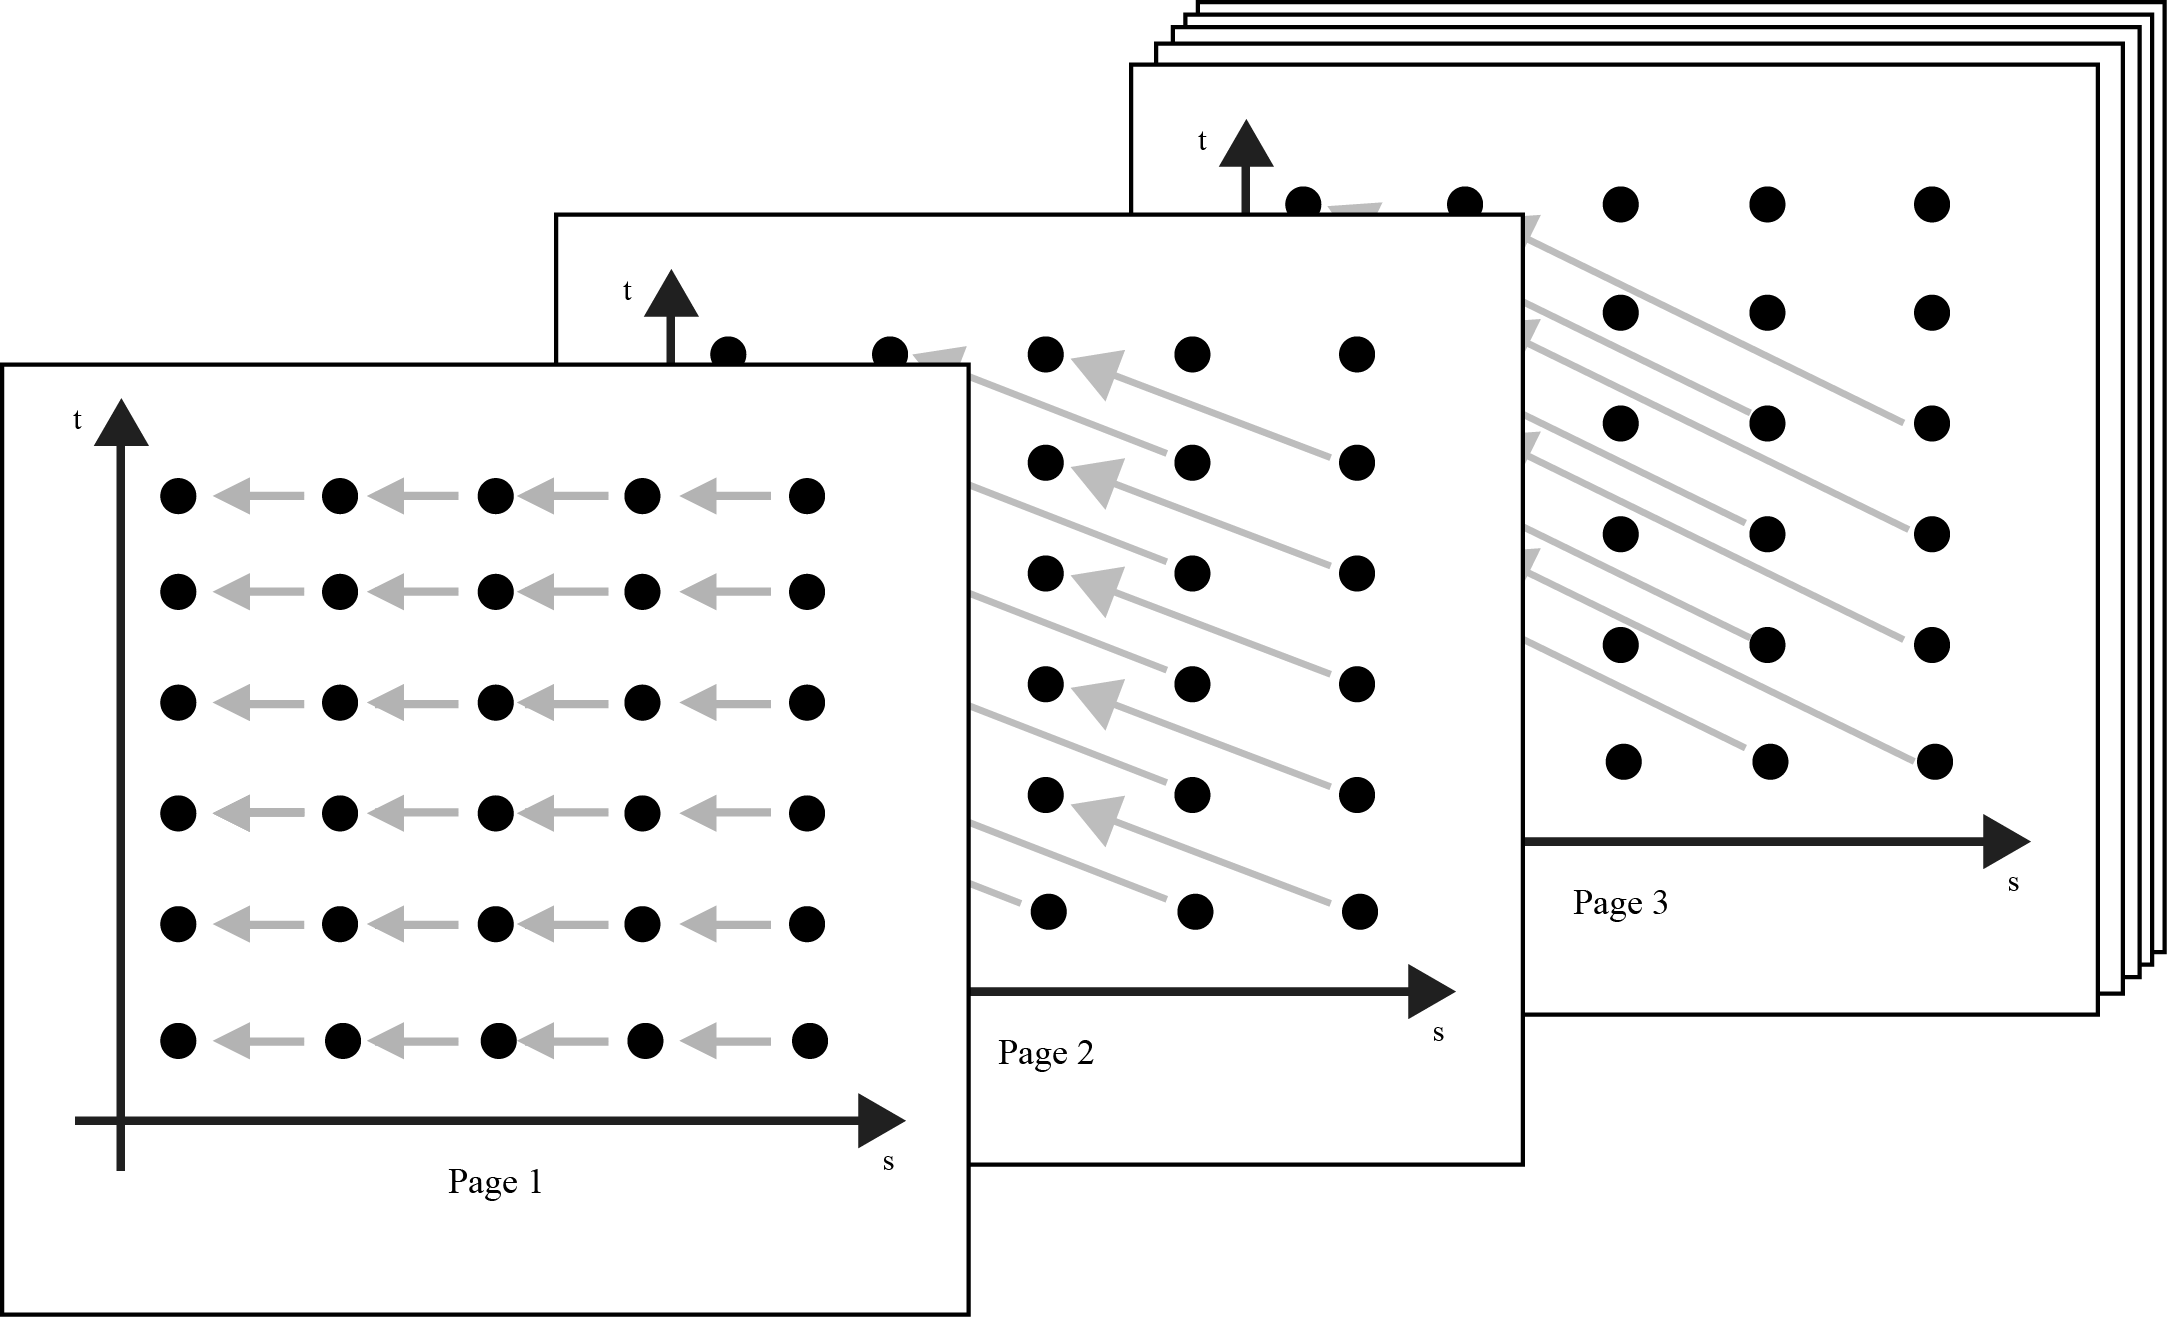
\includegraphics[width=\linewidth,height=0.5\textheight,keepaspectratio]{figures/cover.png}
  \end{center}
       \begin{minipage}{.35\linewidth}
    \begin{flushleft}
      \vspace{2em}
      {\fontsize{6pt}{2pt} \textit{Notes: These are partially live-tex'd
notes from a graduate course in Algebraic Topology taught by Justin
Roberts at the University of California San Diego in Fall 2017. As such,
any errors or inaccuracies are almost certainly my own. } } \\
    \end{flushleft}
    \end{minipage}
    \hfill
    \begin{minipage}{.65\linewidth}
    \end{minipage}
  }







\begin{document}

\date{}
\maketitle
\begin{flushleft}
\textbf{D. Zack Garza} \\
\textit{University of Georgia} \\
\textit{dzackgarza@gmail.com} \\
{\tiny \textit{Last updated:} 2020-10-22 }
\end{flushleft}


\newpage
\tableofcontents

\hypertarget{prologue}{%
\section{Prologue}\label{prologue}}

\hypertarget{references}{%
\subsection{References}\label{references}}

\begin{itemize}
\tightlist
\item
  Hatcher's Algebraic Topology \autocite{hatcher_2019}.
\end{itemize}

\hypertarget{homology}{%
\section{Homology}\label{homology}}

What is homology? Seems to be ubiquitous in mathematics, pops up in
number theory, algebraic geometry, topology (obviously), etc.

Many routes to motivate it, we'll take the topological tact. Coming up:

\begin{enumerate}
\def\labelenumi{\arabic{enumi}.}
\item
  Simplicial Homology

  \begin{itemize}
  \tightlist
  \item
    Of simplicial complexes, a la Poincaré \textasciitilde1900
  \item
    Easier to compute
  \end{itemize}
\item
  Singular Homology

  \begin{itemize}
  \tightlist
  \item
    Easier to define and more general
  \item
    Harder to compute, need theorems
  \end{itemize}
\end{enumerate}

\begin{definition}[$n\dash$simplex]

An \emph{n-simplex} \(\sigma = (a_0, \cdots a_n) \subseteq \RR^n\) is a
\emph{convex hull} of \(n+1\) points when the points are \emph{affinely
independent}.

\end{definition}

The \emph{convex hull} is given by
\begin{align*}
\theset{\sum \lambda_i a_iL \mid 0 \leq \lambda_i \leq 1, \sum \lambda_i = 1}
,\end{align*} i.e.~set of centers of gravity of masses placed at
vertices.

They are affinely independent if there is a unique expression of every
point in barycentric coordinates.

\begin{align*}
\sum v_i a_i = 0 \text{ and } \sum v_i = 0 \implies v_i = 0 ~\forall i
.\end{align*} It follows that
\begin{align*}
\sum \lambda_i a_i = \sum \mu_i a_i
\implies
\lambda_i = \mu_i ~\forall i
\end{align*}

The \emph{face} of an \(n\)-simplex are the subsets where the
barycentric coordinates are 0. Consider a triangle with points
\(\lambda a, \mu b, \nu c\), then one edge is a face (\(\lambda=0\)), as
is another \((\nu = 0\)), as is the point \(\mu b\) where
\(\nu = \lambda = 0\). An \(n\)-simplex has \(2^n - 1\) faces, including
the entire thing (\(2^n - 2\) otherwise)

\begin{definition}[Simplicial Complex]

A \emph{simplicial complex} is a set \(K\) of simplexes in \(\RR^n\),
say \(K = \theset{\sigma_0, \sigma_1 \cdots \sigma_n}\), such that they
are pasted together correctly, i.e.

\begin{enumerate}
\def\labelenumi{\arabic{enumi}.}
\tightlist
\item
  \(\sigma \in K \text{ and } \tau \subset \sigma \implies \tau \in K\)
\item
  If \(\sigma, \sigma' \in K\) then they overlap in a common face,
  i.e.~either
  \(\sigma \intersect \sigma' = \emptyset \text{ or } \sigma\intersect\sigma'\)
  is a face of both \(\sigma,\sigma'\).
\end{enumerate}

\end{definition}

\begin{definition}[Geometric Realization]

Given such a \(K\), its \emph{geometric realization} is given by the
topological space
\begin{align*}
\abs{K} \da \Union_{\sigma\in K} \sigma \subseteq \RR^n
.\end{align*}

\end{definition}

\begin{definition}[Triangulation]

A \emph{triangulation} of a space \(X\) is a homeomorphism
\(h: X \into \abs{K}\) for some \(K\).

\end{definition}

\begin{example}

\(S^1\) is homeomorphic to a triangle, which has 6 total simplexes:
three points \(\Delta_0\), and 3 edges \(\Delta_1\). Similarly, \(S^2\)
is homeomorphic to a tetrahedron with 14 simplexes.

\end{example}

\begin{remark}

We don't want to allow anything particularly curved, or anything with
multiple edges.

\end{remark}

\begin{definition}[Abstract Simplicial Complex]

An \emph{abstract simplicial complex} is a set \(V\) of vertices
together with a set \(K \subset P(V)\) of subsets of \(V\) which is
closed under taking subsets
(\(\sigma \in K \text{ and } \tau \subseteq \sigma \implies \tau \in K\))

\end{definition}

\begin{example}

\(V = \theset{1,2,3,4}\), then the 4-simplex can be described as
\begin{align*}
K = \theset{\theset{1}, \theset{2}, \theset{3}, \theset{4}, \theset{1,2}. \theset{2,3}, \theset{1,3}, \theset{1,2,3}}
.\end{align*}

\end{example}

\begin{definition}[Geometric Realization of a Simplicial Complex]

We have a notion of \emph{geometric realization}: we can embed \(K\)
inside \(\RR^{\abs{V}}\) where each basis vector is in correspondence
with each vertex.

\end{definition}

\begin{remark}

Note that here \(\sigma\) maps to the convex hull of its vertices. The
moral of the story here is that abstract simplicial complexes can be
realized as geometric simplicial complexes.

\end{remark}

\begin{definition}[Orientation of a Simplex]

An \emph{orientation} of a simplex is a choice of ordering of vertices
up to even permutations,
i.e.~\((a,b,c) = (c,a,b) = (b,c,a) \neq (b,a,c) = (c,b,a) = (a,c,b)\).

\end{definition}

\begin{example}

A point is a special case, there are two orientations, \(\pm *\). Take
\(+*\) to be the canonical orientation.

\end{example}

\begin{example}

How does this work in 3 dimensions? Take \((a,b,c,d)\) be an orientation
on a tetrahedron - this is roughly equivalent to choosing an oriented
frame, but there are many interpretations. So just view as equivalence
classes after modding out by even permutations.

\end{example}

\begin{definition}[?]

If \(K\) is a simplicial complex, let \(C_n(K)\) be the free abelian
group on oriented \(n\)-simplexes in \(K\) quotiented by
\(\bar\sigma \sim -\sigma\). Add twice as many simplexes then quotient
out..? Avoids making choices of orientation everywhere! Then each
oriented \(n\)-simplex maps into \(C_n(K)\) in a natural way.

\end{definition}

\begin{definition}[?]

A boundary map \(\bd: C_n K \into C_{n-1} K\) by linearly extending the
formula
\begin{align*}
\bd(a_0 \cdots a_n) = \sum_{i=1}^n (-1)^i (a_0, \cdots \hat{a_i} \cdots a_n)
,\end{align*} where the summand denotes the face spanned by all vertices
except \(a_i\).

\end{definition}

\begin{example}

We can directly compute \(\del (a,b) = (b) - (a)\) and
\(\del(a,b,c) = (b,c) - (a,c) -+(a,b)\). So a line segment
\(a \mapsto b\) goes to \(-a\) and \(+b\). An oriented triangle \(abc\)
goes to the three line segments oriented in the same way.

What happens?

\end{example}

Need to check that \(\bd\) is well defined - check that applying a
transposition, e.g.~\((a_0 a_1)\).

\begin{align*}
\bd (a_1, a_0, a_2, \cdots a_n) = (a_0, a_2, \cdots a_n) - (a_1, a_2, \cdots a_n) + \sum \text{stuff} = -\bd (a_0, a_1, a_2, \cdots a_n)
,\end{align*} so equality is preserved under even permutations.

\begin{proposition}[Simplicial Boundary Map is Well-Defined]

\begin{align*}  
\bd^2 = 0
.\end{align*}

\end{proposition}

Consider
\begin{align*}
C_n K \into_{\del_n} C_{n-1} K \into_{\del_{n-1}} C_{n-2} \into \cdots
\end{align*}

\hypertarget{the-bar-resolution-and-group-homology}{%
\section{The Bar Resolution and Group
Homology}\label{the-bar-resolution-and-group-homology}}

Last time: the Koszul complex and free resolutions. Today: group
homology

\hypertarget{bar-resolutions}{%
\subsection{Bar Resolutions}\label{bar-resolutions}}

Let \(A\) be an associative, unital, generally not commutative algebra
over a field \(k\) (or just a ring over \(\ZZ\)). Consider the category
of \(A\dash A\dash\) bimodules, which has the fundamental structure of
two multiplication maps of the form
\begin{align*}
A\tensor M \tensor A &\to M\\
a_1\tensor m \tensor a_2 &\mapsto a_1 m a_2
\end{align*}

There is a particularly interesting module \({}_A A_A\), the
``diagonal'' or ``trivial'' module. It's trivial because as functors, we
have
\begin{align*}
(\wait)\tensor_A {}_A A_A = \id
.\end{align*}

Note that this module is not free. However, compare this to
\({}_A(A\tensor_k A)_A\). This is a free module, since it is a vector
space over \(k\), of rank 1 with generator \(1\tensor 1\). So we can
write a free resolution of \({}_A A_A\) as a bimodule:

\begin{align*}
(A^{\tensor 4}) 
&\mapsvia{a\tensor b\tensor c \tensor d \mapsto ab\tensor c\tensor d - a\tensor bc \tensor d + a\tensor b \tensor cd} 
{}_A(A^{\tensor 3})_A 
&\mapsvia{f_1:~a\tensor b \tensor c ~\mapsto~ ab\tensor c - a\tensor bc} {}_A(A\tensor_k A)_A 
&\mapsvia{f_0: ~a\tensor b~ \mapsto~ a1b} {}_A A_A \to 0
\end{align*}

Then \(f_1\) surjects onto \(\ker f_0\), yielding the second term.

Continue to yield
\begin{align*}
B^{-n}(A) = {}_A A\tensor_k A^{\tensor_k^{n}}\tensor_k A_A
,\end{align*} which is free as an \(A\dash A\dash\) bimodule since it
decomposes as a direct sum indexed by the middle term.

Then there is a differential
\begin{align*}
B^{-n} &\to B^{-n+1} \tag*{($n \geq -1$)} \\
a_0 \tensor (a_1 \tensor \cdots \tensor a_k) \tensor a_{n+1} 
&\mapsto \sum (-1)^i a_0 \tensor \cdots \tensor a_i a_{i+1} \tensor \cdots \tensor a_{n+1}
\end{align*}

You can check that \(d^2 = 0 \iff A\) is associative. This is something
that works in general -- for example, with lie algebras, the associative
multiplication is replaced by the lie bracket, and the equivalence is to
the Jacobi identity.

\begin{claim}

This is a resolution. Just write down a map
\(A\tensor A \to A\tensor A \tensor A\) that is chain homotopic to the
zero map. Something obvious works: let
\begin{align*}
h(a_0 \tensor \cdots \tensor a_{n+1}) = 1\tensor a_0 \tensor \cdots \tensor a_{n+1}
,\end{align*} then just check that \(dh + hd = \id - 0\).

\end{claim}

\begin{remark}

This is not actually a bunch of maps of bimodules, only of right \(A\)
modules -- but this is enough to show that this complex is acyclic,
i.e.~kernels = images.

\end{remark}

We can define homologies associated to this. One example is the
Hochschild Cohomology with coefficients in a bimodule, denoted
\begin{align*}
HH^*(A;M) \definedas \ext_{A\dash A\dash\text{mod}}^*({}_A A_A, {}_A M_A)
.\end{align*} In other words, take the bar resolution of \(A\), hom it
into \(M\) (\(\hom_{A\dash A}(B^*(A), M))\), and take kernels modulo
images.

Whenever you have a derived functor, the original functor should come up
in the zeroth homology. In this case, it extends to \(HH^0(A, M)\) is
analogous to the ``center'' of \(M\), i.e.~
\begin{align*}
HH^0(A, M) = \theset{m\in M: am = ma, ~\forall a\in A}
.\end{align*}

Also, \(HH_*(A; M) = \tor(A, M)\), and
\begin{align*}
HH_0 = \frac{M}{\gens{am=ma}}
,\end{align*} is the ``cocenter'' of \(M\). This forcibly quotients out
all of the commuting elements!

This resolution is easiest seen over bimodules, but the same basic
complex can be formed in the category of plain left/right modules. So
given \({}_A M \in \mathbf{A\dash mod}\), regard it as
\({}_A A_A \tensor_A M \cong M\) where \(a\tensor m \mapsto am\). Then
\({}_A B(A)_A \tensor_A M\) is still a complex of free \emph{left}
modules that only depends on the module \(A\), so this is a universal
type of resolution.

We can use this to compute things like

\begin{align*}
\ext_{A\dash mod}({}_A M, {}_A A) 
&= h(\shom^*_{A\dash mod}~ ({}_AB^{\leq 0}(A) \tensor_A M, {}_A N)) \\
\tor_{A\dash mod}(N_A, {}_A A) 
&= h(N\tensor_A B^{\leq 0}(A) \tensor_A M)
.\end{align*}

\hypertarget{homology-of-a-discrete-group}{%
\subsection{Homology of a Discrete
Group}\label{homology-of-a-discrete-group}}

Let \(G\) be a discrete group -- note that we could always think of
these of topological spaces, just not in this instance. Let
\(A = \ZZ[G]\) be the group ring: formal finite integer linear sums of
elements in \(G\) with the obvious multiplication.

\begin{remark}

Note that a general \(k\dash\)algebra is not always augmented, so there
is not always a way to make \(k\) into an \(A\) module.

\end{remark}

This algebra is in fact augmented, i.e.~it has an algebra homomorphism
\(\ZZ[G] \mapsvia{\varepsilon} \ZZ\), so we can make \(\ZZ\) into a left
\(A\) module for \(A = \ZZ[G]\) where \(a\in A\) acts on \(n\in \ZZ\) by
\(a.n \mapsto \varepsilon(a)n\).

This allows us to define
\begin{align*}  
H_*(G; M) \definedas \tor_{\ZZ[G]}(\ZZ_{\ZZ[G]}, {}_{\ZZ[G]} M)
.\end{align*} In particular, we could just define
\begin{align*}
H^*(G; \ZZ) \definedas \tor_{\ZZ[G]}(\ZZ_{\ZZ[G]}, {}_{\ZZ[G]} \ZZ)
.\end{align*}

These extend the natural functors, the ``coinvariants'', and
\begin{align*}
H^0(G;M) &= \theset{m\st gm = m} \\
H_0(G; M) &= \frac{M}{\gens{ g.m=m} }
\end{align*}

\textbf{Next Time}

\begin{itemize}
\tightlist
\item
  Explicit chain complex using bar resolutions
\item
  Explicit complexes using the resolution in the case \(G=\ZZ_n\)
\item
  Relation to simplicial classifying spaces.
\end{itemize}

\begin{figure}
\centering
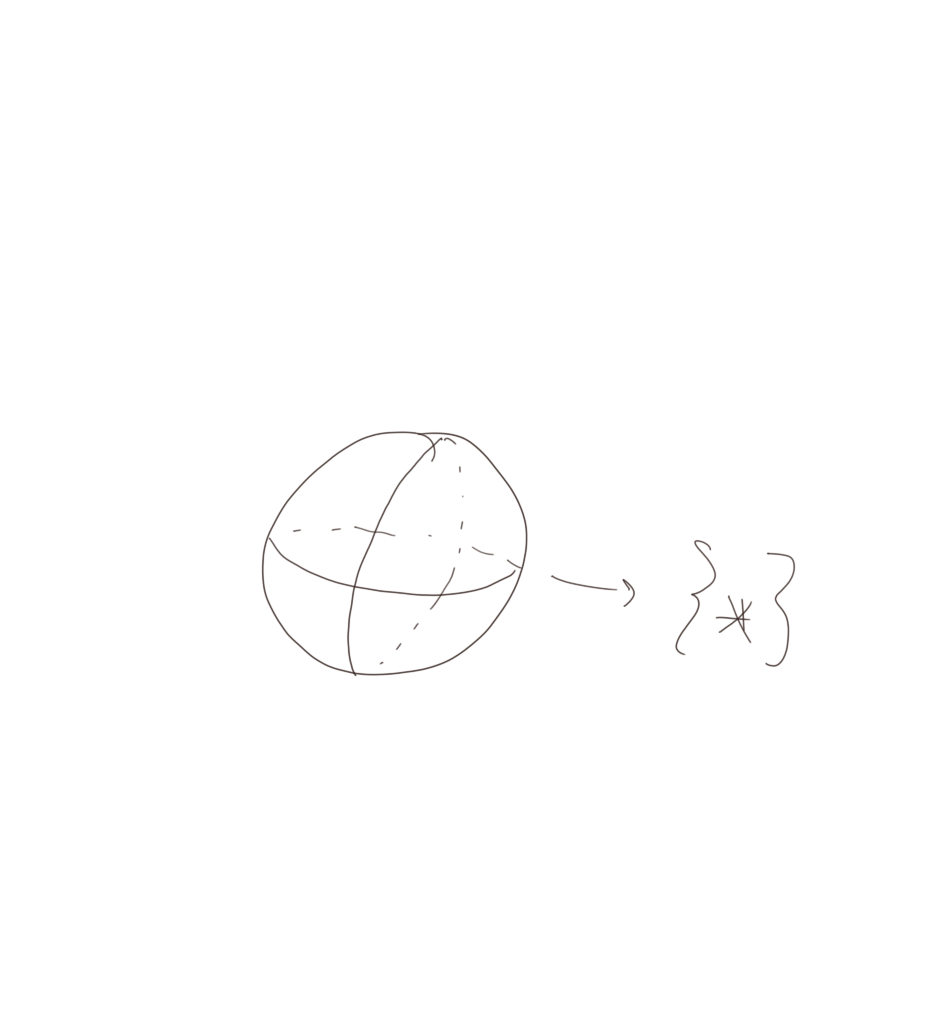
\includegraphics[width=2.60417in,height=\textheight]{figures/2-21-18-b2ad9.png}
\caption{Image}
\end{figure}

\hypertarget{group-homology}{%
\section{Group Homology}\label{group-homology}}

Let \(G\) be a discrete group and \(A=\ZZ[G]\) a group ring, and
consider the category of \(A\dash\)modules.

We can define the trivial module \({}_{\ZZ[G]}\ZZ\) where \(g\) acts by
1 for all \(g\in G\). This has to come equipped with a homomorphism
\begin{align*}
\ZZ[G] &\mapsvia{\varepsilon} \ZZ \\
g &\mapsto 1
\end{align*}

\begin{example}

Take \(G=\ZZ_2\) and \(A = \ZZ[\ZZ_2]\) which is equal to
\begin{align*}
\ZZ[x] / (x^2-1) = \theset{a + bx\mid a,b\in \ZZ, x^2=1}
.\end{align*} Construct by hand a resolution of \({}_{A}\ZZ\) -- this
will require some choices, but this will be alright as long as they are
reasonably constrained and uniform, i.e.~there isn't some infinite
process of choices.

Given an algebra, we can think of it as a bimodule over itself (not
free), so we can always use the bar resolution. But in this case, that
may be too big!

So look at
\begin{align*}
\ZZ/(x^2-1).e_2 \mapsvia{e_2 \mapsto (x+1).e_1} \ZZ/(x^2-1) \mapsvia{e_1 \mapsto (x-1)e_0} \ZZ \to 0
.\end{align*} Note that the polynomials just act by evaluation at 1, so
there are several different ways of looking at the indicated map - one
of which is just to send the generator to 1.

So the kernel if this map actually is the ideal \((x-1)\). Think of
elements
\begin{align*} 
(a+bx).e_0 = (a+bx)(1) = a+b
,\end{align*} so the kernel is generated by elements \(a=b\), or
equivalently the ideal \((x-1)\). A similar pattern continues as you
resolve, which is periodic -- note that \(e_3 \mapsto (x-1).e_2\). So
picking the minimal thing worked, which ended up having a 2-periodic
pattern -- so relatively simple to work with.

So this 2-periodic free resolution can be used
\begin{align*}
\bar A = \qty{ \cdots A \mapsvia{x(x-1)} A \mapsvia{x(x+1)} A \mapsvia{x(x-1)} \cdots}
\end{align*}

From this we can compute \(\tor_*^{\ZZ[G]} (\ZZ, \ZZ)\), which is by
definition \(H_*(G;\ZZ)\). But working this out, we find it is equal to
\(h(\bar A \tensor \ZZ)\). Use the isomorphism

\begin{align*}
A\tensor_A \ZZ \mapsvia{a\tensor 1 \mapsto \varepsilon(a)1} \ZZ
.\end{align*} Note that \(\varepsilon(x-1) =0\) and
\(\varepsilon(x+1) = 2\), so we have

\begin{align*}
h(\cdots \mapsvia{\times 2} \ZZ \mapsvia{\times 0} \ZZ \mapsvia{\times 2} \ZZ \cdots)
.\end{align*} Thus we have
\(H_*(\ZZ_2, \ZZ) = \ZZ \delta_0 + \ZZ_2 \delta_{\text{odd}}\).

\begin{quote}
Note that this is equal to \(H_*(\RP^\infty; \ZZ)\)!
\end{quote}

\end{example}

\begin{example}

Similarly, we can do this for \(\ZZ_n\), looking at
\(A = \ZZ[x] / (x^n - 1)\), yielding a similar resolution:
\begin{align*}
\cdots A \mapsvia{\times(x-1)} A \mapsvia{\times(1+x+\cdots x^{n-1})} A \mapsvia{\times (x-1)}A \to \ZZ \to 0
\end{align*} Delete the right hand side, tensor this over \(\ZZ\) to
yield
\begin{align*}
\cdots A \mapsvia{\times n} A \mapsvia{\times 0} A \mapsvia{\times n} A \cdots
\end{align*} This is equal to \(H_*(L^\infty_n; \ZZ)\), which is equal
to \(S^{2n-1} / \ZZ_n\) which can be constructed in a CW fashion. This
is an interesting space which is contractible, but not a point -- note
that there is a free action on it via \(\ZZ_n\) which has no fixed
points, so it's ``big''.

\end{example}

So this allows us to look at groups as spaces of some sort.

It turns out that there is a universal way to resolve any
\(\ZZ[G]\dash\)module. Look at

\begin{align*}
\bigoplus_{h\in G} \ZZ[G].e_h \mapsvia{} \ZZ[G] \mapsvia{g\mapsto 1} \ZZ \to 0
\end{align*}

What is the kernel of the first map? It is
\(\ZZ\theset{g-1\mid g\in G}\)

Switch up the notation, and write it like a free resolution of abelian
groups
\begin{align*}
\ZZ[G^3] \mapsvia{(g,h,k) \mapsto (g-h) + (h-k) + (k-g)} \ZZ[G^2] \mapsvia{(g,h) \mapsto g-h} \ZZ[G] \mapsvia{g\mapsto 1} \ZZ \to 0
\end{align*}

We can then define a complex \(C_n = \ZZ[G^n]\) of free abelian groups
that is acyclic, using
\begin{align*}
\del((g_0, g_1, \cdots g_n)) = \sum (-1)^i (g_0, \cdots \bar g_i, \cdots g_n)
\end{align*}

You can write down a contracting homotopy, as in the case of the bar
complex, as
\begin{align*}
h(g_0 \cdots g_n) \mapsto (1, g_0, \cdots g_n)
  \end{align*}

This is a chain homotopy between the identity map and the zero map,
i.e.~\(\del h + h\del = \id - 0\), so the induced map on homology by the
identity is equal to the induced map on homology by the zero map - thus
zero homology.

In the bar complex, we only acted on the boundary terms and the middle
didn't play much of an algebraic role. This is a complex of left
\(G\dash\)modules if we use the diagonal action of \(G\), where
\(g.(g_0, \cdots g_n) = (gg_0, \cdots , gg_n)\).

So to compute \(H_*(G; \ZZ)\), we want to tensor with a right module so
we take \(\tor_*^{\ZZ[G]}(\ZZ_n, {}_n \ZZ)\), where the right slot has
already been resolved.

We identify, although this isomorphism must be handled carefully - we
don't want to make \(g_0\) a privileged choice in a map like
\begin{align*}
\ZZ \tensor_{\ZZ[G]} \ZZ[G^{n+1}] \cong \ZZ[G^n]
\end{align*}

\begin{align*}
(g_0, g_1, \cdots g_n) \mapsto (1, g_1g_0^{-1}, \cdots g_ng_0^{-1}).\end{align*}

It's better to label by the differences, i.e.~
\begin{align*}
(g_0, g_1, g_2, \cdots) = (g_0, g_0^{-1}g_1, g_1^{-1}g_2, \cdots)
,\end{align*} which is a \(g_0\) invariant sort of notation.

This is the resolution usually seen in books, i.e.~you might see
\begin{align*}
\del(g_1, g_2, \cdots g_n) = (g_2, \cdots g_n) + \sum (-1)^i (\cdots ,g_i g_{i+1}, \cdots) + \cdots
\end{align*}

\hypertarget{intersection-theory}{%
\section{Intersection Theory}\label{intersection-theory}}

Goal: we'd like a geometric interpretation of the cup product.

Recall that we had an idea of representing homology classes in a space
\(X\) by maps from a closed connected manifolds \(f: P \to X\). We can
then take the push forward of a fundamental class

\begin{align*}
f_*[P] \in H_p(X; \ZZ) \text{ where } [P] \in H_p(P)
\end{align*}

\begin{remark}

The best case is when \(X = M^n\) is a closed \(n\dash\)dimensional
closed manifold and \(f\) is the inclusion of a \emph{locally flat
submanifold}.

\end{remark}

\begin{definition}[?]

A subset of \(P \subseteq M^n\) which is locally homeomorphic to
\(\RR^p\) is a \emph{locally flat submanifold} if at every point
\(x\in P\) there exists a neighborhood \(U\) of \(x\) in \(M\) and a
homeomorphism
\begin{align*}\phi: (U, U\cap P, x) \to (\RR^n, \RR^p \cross \theset{0}, \theset{0})\end{align*}.

\end{definition}

\begin{warning}

An example of a non locally flat submanifold: take the trefoil knot
\(K\) in \(S^3 \subset B^4\) and cone it to the origin to produce
\(CK\). This fails local flatness at the origin, despite the fact that
\(CK \cong B^2\). Every neighborhood of the origin contains a copy of
\(K\) and \textbf{not} a copy of \(S^1 \in S^3\) unknotted. In general,
the operation of taking a cone on a smooth manifold will not produce a
smooth manifold - but in the topological world, sometimes this works
out.

\end{warning}

\begin{example}

Consider the Poincaré 3-sphere \(P^3\), which has the same homology as
\(S^3\). Even though \(\Sigma P^3\) may not be a manifold a priori, we
actually have \(\Sigma^2 P^3 \cong S^5\).

\end{example}

Note that while we may expect two \(p\dash\) dimensional submanifolds to
just intersect in some number of points (e.g.~a curve intersecting a
torus inside \(B^4\) or something), but there may be some degenerate
cases: they might be tangent, or part of one may lie inside the other.

\begin{definition}[Locally Flat Submanifolds]

If \(P^p, Q^q\) are locally flat submanifolds of \(M\), we say that they
\emph{intersect transversally} \(P \pitchfork Q\) when:

\begin{enumerate}
\def\labelenumi{\arabic{enumi}.}
\item
  Case 1 \(p+q < n \implies P \cap Q = \emptyset\)
\item
  Case 2 \(p+1 \geq n\) then we require that \(\forall x\in P \cap Q\),
  there exists a local neighborhood \(U \subset M\) and a homeomorphism
  \begin{align*}\phi: (U, U\cap P\cup Q, x) \to (\RR^n, \RR^p \cross \theset{0} \cup \theset{0} \cross \RR^q, \theset{0})\end{align*}
\end{enumerate}

\begin{quote}
Note: this ensures that \(P\cap Q\) is a \((p+q-n)\dash\)manifold.
\end{quote}

\end{definition}

\begin{remark}

For vector spaces \(X, Y \subset V\) where \(p,q \leq n\), we can then
say they are transverse exactly when \(X \oplus Y = V\) (so \(X, Y\)
span \(V\)). This is primarily because
\(\dim (X \cap Y) = \dim X + \dim Y - \dim(X\oplus Y)\). In the case of
smooth manifolds, you might actually use this as a definition: two
manifolds intersect transversally iff their tangent planes span the
ambient tangent space.

\end{remark}

\begin{remark}

If we had smooth manifolds \(P, Q\) (i.e.~differential topology), then
Sard's theorem plus extra work would show that there exist arbitrarily
small perturbations of \(P, Q\) such that \(P \pitchfork Q\).

\end{remark}

\begin{example}

Consider a parabola hitting a plane at a point. Move one way to make
disjoint, get empty set intersection -- this trivially satisfies
conditions of transversality. You can move this slightly to make it
intersect exactly twice.

\end{example}

This makes certain degenerate cases easier - i.e.~a curve intersecting a
plane in an interval, or doing something like \(\sin(1/x)\) on a
surface.

The number of points of intersection is not exactly a homotopy
invariant, since in the above example we could make the intersection
number either 2 or 0. However, the \emph{parity} can be proved to be
such an invariant in the smooth setting. This leads into Morse theory.
For example, look at cubic intersecting plane -- perturbations will
coalesce two intersection points, which would be a Morse critical point.

In this world, you'll have vocabulary available

\begin{itemize}
\tightlist
\item
  Generic
\item
  Stable
\item
  Regular
\item
  Transverse
\item
  Random
\end{itemize}

\begin{example}

For example, look at \(\mathcal{M} = [S^1, \RR^3]\). Transverse maps are
an open and dense subset of this parameter space. Imagine as blob cut up
by ``walls'' which are the closed subsets of bad maps. Not only are the
good maps dense, but they are stable -- everything in a small enough
neighborhood will also be good. A random map picked from this space will
be good with probability 1.

Two such maps can be generically homotoped without hitting the
intersection of the singular walls, i.e.~just going through walls with
no intersection points). This ultimately just boils down to looking at
Taylor series - generically, the first coefficient is nonzero, so
intersects \(x\dash\)axis transversally. If not, the second coefficient
is probably nonzero, so intersects quadratically, etc.

\end{example}

\begin{theorem}[?]

If \(P^p, Q^q\) are transverse in \(M^n\) where \(p+q=n\) (and
everything closed and oriented), then
\begin{align*}
\#(P \cap Q)= \inner{D^{-1}[P] \smile D^{-1}[Q]}{ [M] }
,\end{align*} where the first entry is a cup product between
\(H^q(M; \ZZ)\) and \(H^p(M; \ZZ)\). This is an algebraic and homotopy
invariant on the RHS, and geometric on the LHS.

\end{theorem}

\hypertarget{relative-homology}{%
\section{Relative Homology}\label{relative-homology}}

Continuing discussion of relative homology:
\begin{align*}
H_*(X,A) = H(C_* X/ C_* A)
\end{align*}

When axiomatized, generally relies on property of \textbf{excision},
which relates to the following theorem:

\begin{theorem}[?]

If \(U \subseteq A \subseteq X\) and \(cl(U) \subseteq int(A)\), then
\begin{align*}
H(X, A) \cong H(X-U, A-U)
\end{align*} or equivalently setting \(X = A \union B\) where
\(X = int(A) \union int(B)\), then
\begin{align*}
H(X,A) \cong H(B, A\intersect B)
\end{align*}

\end{theorem}

\begin{proof}

Recall from proof of Mayer Vietoris we used
\begin{align*}
C_*(A+B) \leq C_* X = \ts{\text{singular simplexes from } A \text{ or } B}
\end{align*} This yields a SES
\begin{align*}
    0 \mapsvia{} C_*(A) \mapsvia{} C_*(A+B) \mapsvia{} C_*(B, A\intersect B)\mapsvia{} 0
    \end{align*}

Look at inclusion \(C_*(A+B) \mapsvia{\iota} C_*(X)\) and its placement
in the SES
\begin{align*}
0\mapsvia{} C_*(A) \mapsvia{} C_*(X) \mapsvia{} C_*(X,A)\mapsvia{} 0
\end{align*} These yield commuting long exact sequences:

\begin{align*}
H_n(A) \mapsvia{} H_n(A+B) \mapsvia{} H_n(A, A\cap B) \mapsvia{} H_{n-1}(A) \mapsvia{} H_{n-1}(A+B) \mapsvia{} \cdots
\end{align*}

\begin{align*}
H_n(A) \mapsvia{} H_n(X) \mapsvia{} H_n(X,A) \mapsvia{} H_{n-1}(A) \mapsvia{} H_{n-1}(X) \mapsvia{} \cdots
\end{align*}

Here the 5 lemma applies, since there are two maps that are
identifications and \(H_*(A+B) \cong H_*(X)\) by Mayer-Vietoris.

\end{proof}

\begin{example}

Look at \emph{local homology}, i.e.~look at \(H_*(X, X-\{*\})\), this is
equivalent to \(H_*(U, U-\{*\})\) for \textbf{any} open neighborhood
\(U\supseteq \{*\}\). Take any open \(V \subseteq \RR^n\) as an example,
then
\begin{align*}
H_*(V,V-\pt) \cong H_*(U, U-\pt)
\end{align*} for \(U\) an epsilon ball around the point, but then by
homeomorphism this is equal to
\begin{align*}
H_*(\RR^n, \RR^n - \pt) = \ZZ\indic{\text{dim} = n}
\end{align*}

\end{example}

\begin{remark}

This is a stronger statement than ``Brouwer's Invariance of Domain'',
because this invariant picks up the dimension \(n\).

Note that this invariance is given by the following statement: no open
set of \(\RR^n\) can be homeomorphic to a subset of \(\RR^m\) for
\(m\neq n\).

\end{remark}

This can be used to show that e.g.~singular points are weird, e.g.~if
this doesn't yield \(\ZZ\) everywhere in a space \(X\) then \(X\) can
not be a manifold.

\hypertarget{collapsing-theorem}{%
\subsection{Collapsing Theorem}\label{collapsing-theorem}}

If \(X \supseteq A\) and \(A\) has an open neighborhood \(V\supseteq A\)
which deformation retracts onto it then
\(H_*(X,A) \cong \tilde H_*(X/A)\).

Aside:

\begin{definition}[Deformation]

A \emph{deformation} is given by \(A \injects_i V \surjects_p A\) where
\(p\circ i = \id_A\)

\end{definition}

\begin{definition}[Deformation Retract]

A \emph{deformation retract} is given by
\(V \surjects_p A \injects_i V\) where \(i\circ p \homotopic \id_V\)

\end{definition}

\begin{proof}

Take a homeomorphism
\begin{align*}
(X-A, V-A) \cong (X/A - A/A, V/A - A/A)
\end{align*} by homeomorphisms of each component.

By excision, the LHS is isomorphic to \(H_*(X, V)\), while the RHS is
given by
\begin{align*}
H_*(X/A - \pt, V/A - \pt) \cong H_*(X/A, V/A)
\end{align*}

Yields LES of triple
\begin{align*}
0=H_n(V,A) \mapsvia{} H_n(X, A) \mapsvia{} H_n(X,V) \mapsvia{} H_{n-1}(V,A) = 0
\end{align*} so \(H_n(X,A) \cong H_n(X,V)\).

So the RHS is equal to
\begin{align*}
H_*(X/A, V/A) = H_*(X/A, A/A) = H_*(X/A, \pt) = \tilde H_*(X/A)
\end{align*}

\end{proof}

Note that the collapsing argument doesn't work for local homology.

\begin{example}

Consider
\begin{align*}
H_*(\RR^n, \RR^n - \pt) \not\cong \tilde H_*(\RR^n/\RR^n - \pt)
.\end{align*} The LHS depends on \(n\) while the RHS doesn't. Note also
the weird quotient topology on the RHS.

\end{example}

\hypertarget{cellular-homology}{%
\subsection{Cellular Homology}\label{cellular-homology}}

If \(X\) is a CW-complex, then let \(X^n\) be the \(n\)-skeleton. We can
then define
\begin{align*}
C_n^{\text{cell}}(X) \definedas H_n(X^n, X^{n-1}) \cong H_n(X^n/X^{n-1}) \cong \bigvee_{\alpha \in I^n} S_\alpha^n = \bigoplus_\alpha \ZZ
.\end{align*}

Can now introduce a boundary map \(\del:C_n \into C_{n-1}\) from
\begin{align*}
\delta: H_n(X^n, X^{n-1}) \into H_n(X^{n-1}, X^{n-2})
\end{align*} obtained from the LES of the triple
\((X^n, X^{n-1}, X^{n-2})\).

Why is this a chain complex? Does \(\del^2 = 0\)?

Look at \([z] \in H_n(X^n, X^{n-1})\). Then \(z\in C_n(X)\) is a
singular \(n\) simplex, must be a cycle such that
\begin{align*}
\del z \in C_{n-1}X^{n-1} \subseteq C_{n-1}X^n
\end{align*} Then
\begin{align*}
\delta([z]) = [\del z] \in C_{n-1}(X^{n-1}) / C_{n-1}(X^{n-2})
\end{align*} Note the distinction between actual cycles and relative
cycles. But then
\begin{align*}
[\del \del z] = [0] \in H_{n-1}(X^{n-2}, X^{n-3})
\end{align*}

Makes the problem tractable, yields integer linear algebra for finite CW
complexes! This makes things easier to actually compute.

\newpage

\newpage
\section{Indices}
\listoftodos[List of Todos]

% Hook into amsthm environments to list them.
\renewcommand{\listtheoremname}{Definitions}
\listoftheorems[ignoreall,show={definition}, numwidth=3.5em]

\renewcommand{\listtheoremname}{Theorems}
\listoftheorems[ignoreall,show={theorem,proposition}, numwidth=3.5em]

\renewcommand{\listtheoremname}{Exercises}
\listoftheorems[ignoreall,show={exercise}, numwidth=3.5em]

\listoffigures


\printbibliography[title=Bibliography]


\end{document}
